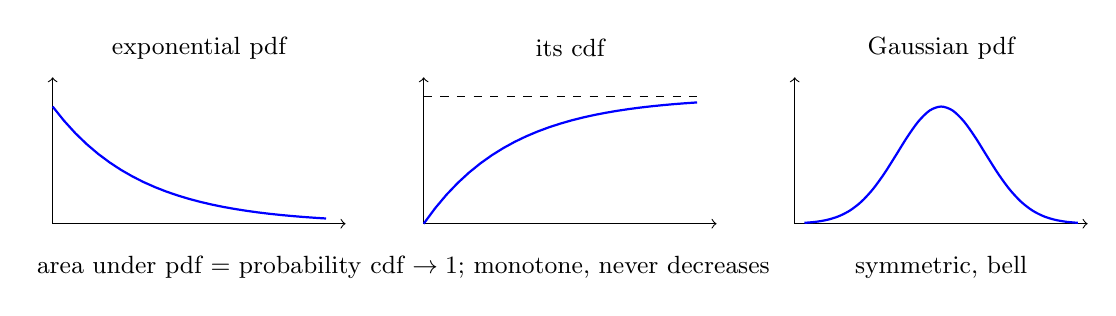
\begin{tikzpicture}[scale=0.62]
% exponential pdf & cdf
\node at (3,3.6) {\small exponential pdf};
\draw[->] (0,0)--(6,0);
\draw[->] (0,0)--(0,3);
\draw[domain=0:5.6,thick,blue] plot (\x,{2.4*exp(-\x/1.8)});
\node at (3,-0.9) {\small area under pdf $=$ probability};
\begin{scope}[xshift=7.6cm]
\node at (3,3.6) {\small its cdf};
\draw[->] (0,0)--(6,0);
\draw[->] (0,0)--(0,3);
\draw[domain=0:5.6,thick,blue] plot (\x,{2.6*(1-exp(-\x/1.8))});
\draw[dashed] (0,2.6)--(5.6,2.6);
\node at (3,-0.9) {\small cdf $\to1$; monotone, never decreases};
\end{scope}
\begin{scope}[xshift=15.2cm]
\node at (3,3.6) {\small Gaussian pdf};
\draw[->] (0,0)--(6,0);
\draw[->] (0,0)--(0,3);
\draw[domain=0.2:5.8,smooth,thick,blue] plot (\x,{2.4*exp(-((\x-3)^2)/1.6)});
\node at (3,-0.9) {\small symmetric, bell};
\end{scope}
\end{tikzpicture}
